\chapter{Inleiding}

\section{Situering}\label{sec:situering}

UML\cite{RumbaughJames2005Tuml} is een visuele modelleertaal geschikt voor algemene doeleinden. Men gebruikt het om artefacten van een softwaresysteem te specificeren en te visualiseren. Deze artefacten bekijken een softwaresysteem vanuit verscheidene oogpunten, en het is de ambitie van UML om genoeg soorten artefacten aan te bieden om een volledige beschrijving te geven van een softwaresysteem. Met behulp van deze artefacten kan men een softwaresysteem ontwerpen en begrijpen.

Wanneer tijdens het modelleerproces het aantal artefacten toeneemt en als individuele artefacten complex worden, wordt het echter moeilijk om een overzicht te behouden van de structuur van het systeem en hoe de componenten van het systeem zich gedragen. Het kan dat men moeilijk die structuur en dat gedrag begrijpt. Tijdens het modelleren kunnen er ook beslissingen worden genomen die ervoor zorgen dat het systeem onmogelijk kan functioneren als het wordt ge\"implementeerd zoals beschreven in de artefacten. Een beslissing kan er ook toe leiden dat een systeem ongewenst gedrag vertoont. Daarom bekijken we in deze masterproef of we voor enkele soorten artefacten, met name klassediagrammen en sequentiediagrammen, gereedschap kunnen aanbieden die de modelleerder helpt om beter inzicht te verkrijgen in wat hij modelleert.

Voor klassediagrammen willen we nagaan:

\begin{itemize}
	\item Of de structuur van een klassediagram niet zo is dat het eigenlijk onmogelijk is om te implementeren.
	\item Of een klassediagram redundante informatie bevat of op zulk een manier gestructureerd is die het moeilijker maakt om het diagram te begrijpen.
\end{itemize}

Voor sequentiediagrammen willen we nagaan:

\begin{itemize}
	\item Of we het gedrag beschreven in sequentiediagrammen kunnen simuleren.
	\item Of we automatisch kunnen controleren of dat gedrag beantwoordt aan bepaalde functionele eisen op het softwaresysteem.
\end{itemize} 

We bouwen zulk een gereedschap op door klassediagrammen en sequentiediagrammen voor te stellen in FO($\cdot$), een uitbreiding van eerste-orde-predicatenlogica. We kiezen voor FO($\cdot$) in de plaats van eerste-orde-predicatenlogica of een meer restrictieve taal omwille van de expressiviteit. Inductieve definities in het bijzonder spelen een cruciale rol bij het voorstellen van sequentiediagrammen.

Sectie \ref{sec:uml-artifacts} geeft een overzicht van de artefacten die UML aanbiedt. Sectie \ref{sec:intro-idp} geeft een inleiding tot IDP\cite{DeCatBroes2014PLaa}, een kennisbanksysteem voor FO($\cdot$). Sectie \ref{sec:research-q} overloopt de probleemstellingen die we bekijken in deze masterproef. Sectie \ref{sec:text-structure} geeft het verdere verloop van deze tekst en beschrijft de bijdragen geleverd in deze masterproef.

\section{Overzicht van UML-artefacten}\label{sec:uml-artifacts}

James Rumbaugh et al.\cite{RumbaughJames2005Tuml} geven een informele indeling van de soorten artefacten in vier domeinen: Het structureel domein; het dynamisch domein; het fysisch domein; en het domein van het modelbeheer. De volgende subsecties geven een kort overzicht van elk domein.

\subsection{Structureel domein}

Artefacten in het structureel domein bekijken het softwaresysteem vanuit de volgende oogpunten:

\begin{itemize}
	\item Het statisch oogpunt: Hieronder vallen klassediagrammen. Klasses zijn modelelementen die discrete stukken informatie bevatten in de vorm van attributen. Ze defini\"eren ook bewerkingen en er wordt ook gespecificeerd met welke andere klasses ze in verband staan door middel van associaties.
	\item Het ontwerpoogpunt: Hieronder vallen interne structuurdiagrammen, collaboratiediagrammen en componentdiagrammen.
	\begin{itemize}
		\item Interne structuurdiagrammen beschrijven voor een bepaalde klasse gedefinieerd in een klassediagram de interne structuur in meer detail.
		\item Collaboratiediagrammen geven weer hoe individuele objecten kunnen samenwerken om een deel van de functionaliteit van de software te bewerkstelligen.
		\item Componentdiagrammen handelen over componenten. Componenten stellen modulaire delen van een systeem voor die extern zichtbare stukken hebben. Deze stukken zijn ofwel functionaliteit die de component aanbiedt gelabeld met een naam, genaamd \textit{interfaces}, ofwel een poort gelabeld met de naam van een \textit{interface}. Een poort kan verbonden worden met een corresponderende \textit{interface} van een andere component. Componentdiagrammen geven weer hoe componenten met elkaar worden verbonden om op hoog niveau het gedrag van een deel van het systeem te specificeren.
	\end{itemize}
	\item Het \textit{use case} oogpunt: Hieronden vallen \textit{use case} diagrammen. Deze diagrammen benoemen verscheidene actoren, die concrete personen of externe systemen kunnen zijn, en geven grafisch weer welke actoren een rol spelen bij welke \textit{use cases}. De ontwerper geeft elders een tekstuele beschrijving voor elke \textit{use case}. Een \textit{use case} beschrijft een concrete dienst die een systeem aanbiedt en benoemt de relevante actoren.
\end{itemize}

Aangezien deze masterproef onder andere handelt over klassediagrammen, geven we hier een klein voorbeeld. Beschouw volgend klassediagram:

\begin{figure}[H]
	\label{fig:cd}
	\centering
	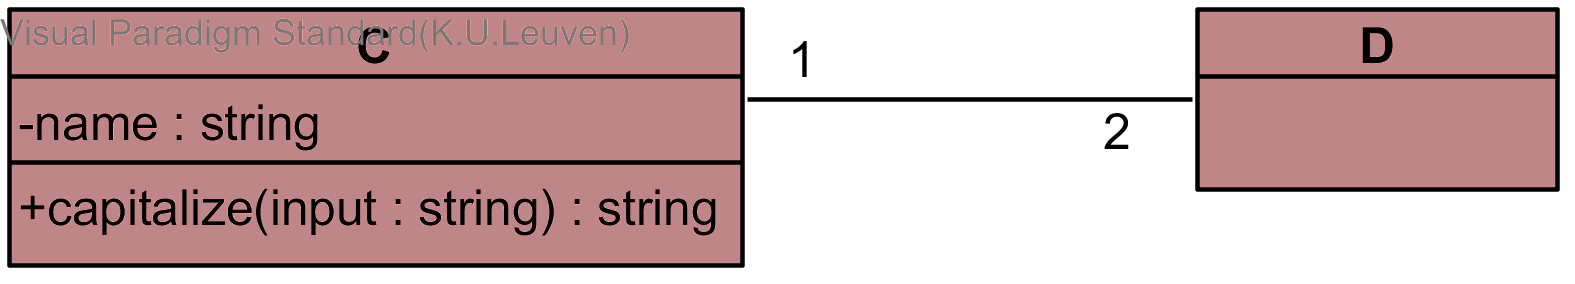
\includegraphics{intro/cd.png}
	\caption{Een voorbeeld van een klassediagram}
\end{figure}

Dit klassediagram drukt uit dat er twee klasses bestaan: \textit{C} en \textit{D}. \textit{C} heeft \'e\'en attribuut, \textit{name}, dat van type \textit{string} is. \textit{D} heeft ook \'e\'en attribuut, \textit{number}, van type \textit{int}. \textit{C} heeft ook \'e\'en operatie \textit{getDNumber} dat \textit{index}, van type \textit{int}, als parameter heeft. \textit{getDNumber(int)} geeft een resultaat terug dat ook van type \textit{int} is. Voorts drukt de lijn tussen \textit{C} en \textit{D} uit dat er een relatie bestaat tussen de twee klasses. Beschouw klasse C. Als we vanuit die klasse de lijn volgen, zien we dat er aan het ander uiteinde staat dat elke \textit{C}-object in relatie moet staan tot exact twee \textit{D}-objecten. Zo ook zien we dat, als we vertrekken vanuit \textit{D}, elk \textit{D}-object in relatie moet staan tot exact \'e\'en \textit{C}-object.

\subsection{Dynamisch domein}

Artefacten in het dynamisch domein bekijken het softwaresysteem vanuit de volgende oogpunten:

\begin{itemize}
	\item Het toestandsautomaatoogpunt: Hieronder vallen toestandsautomaatdiagrammen. Deze diagrammen benoemen toestanden waarin het systeem zich kan bevinden en de mogelijke overgangen tussen de toestanden.
	\item Het activiteitsoogpunt: Hieronder vallen activiteitsdiagrammen. Deze diagrammen beschrijven hoe de besturingsstroom van het systeem kan verlopen tussen activiteiten. Activiteiten zijn processen die bestaan in het systeem.
	\item Het interactieoogpunt: Hieronder vallen sequentiediagrammen en communicatiediagrammen.
	\begin{itemize}
		\item Sequentiediagrammen beschrijven een tijdverloop van een interactie tussen objecten die instanties zijn van klasses gedefinieerd in een klassediagram. Deze diagrammen beschrijven hoe de toestand van \'e\'en of meerdere objecten verandert ten gevolge van een oproep van een methode gedefinieerd voor de klasse waar een bepaald object een instantie van is. Indien de methode een resultaat heeft, wordt ook getoond hoe het resultaat wordt berekend.
		\item Communicatiediagrammen zijn gelijkaardig aan sequentiediagrammen, maar in plaats van het tijdverloop centraal te stellen tonen ze expliciet hoe de objecten betrokken in een oproep met elkaar in verband staan. 
	\end{itemize}
\end{itemize}

Aangezien sequentiediagrammen het tweede soort diagram zijn dat we beschouwen in deze masterproef, geven we ook daar een klein voorbeeld van. Beschouw volgend sequentiediagram:

\begin{figure}[H]
	\label{fig:sd}
	\centering
	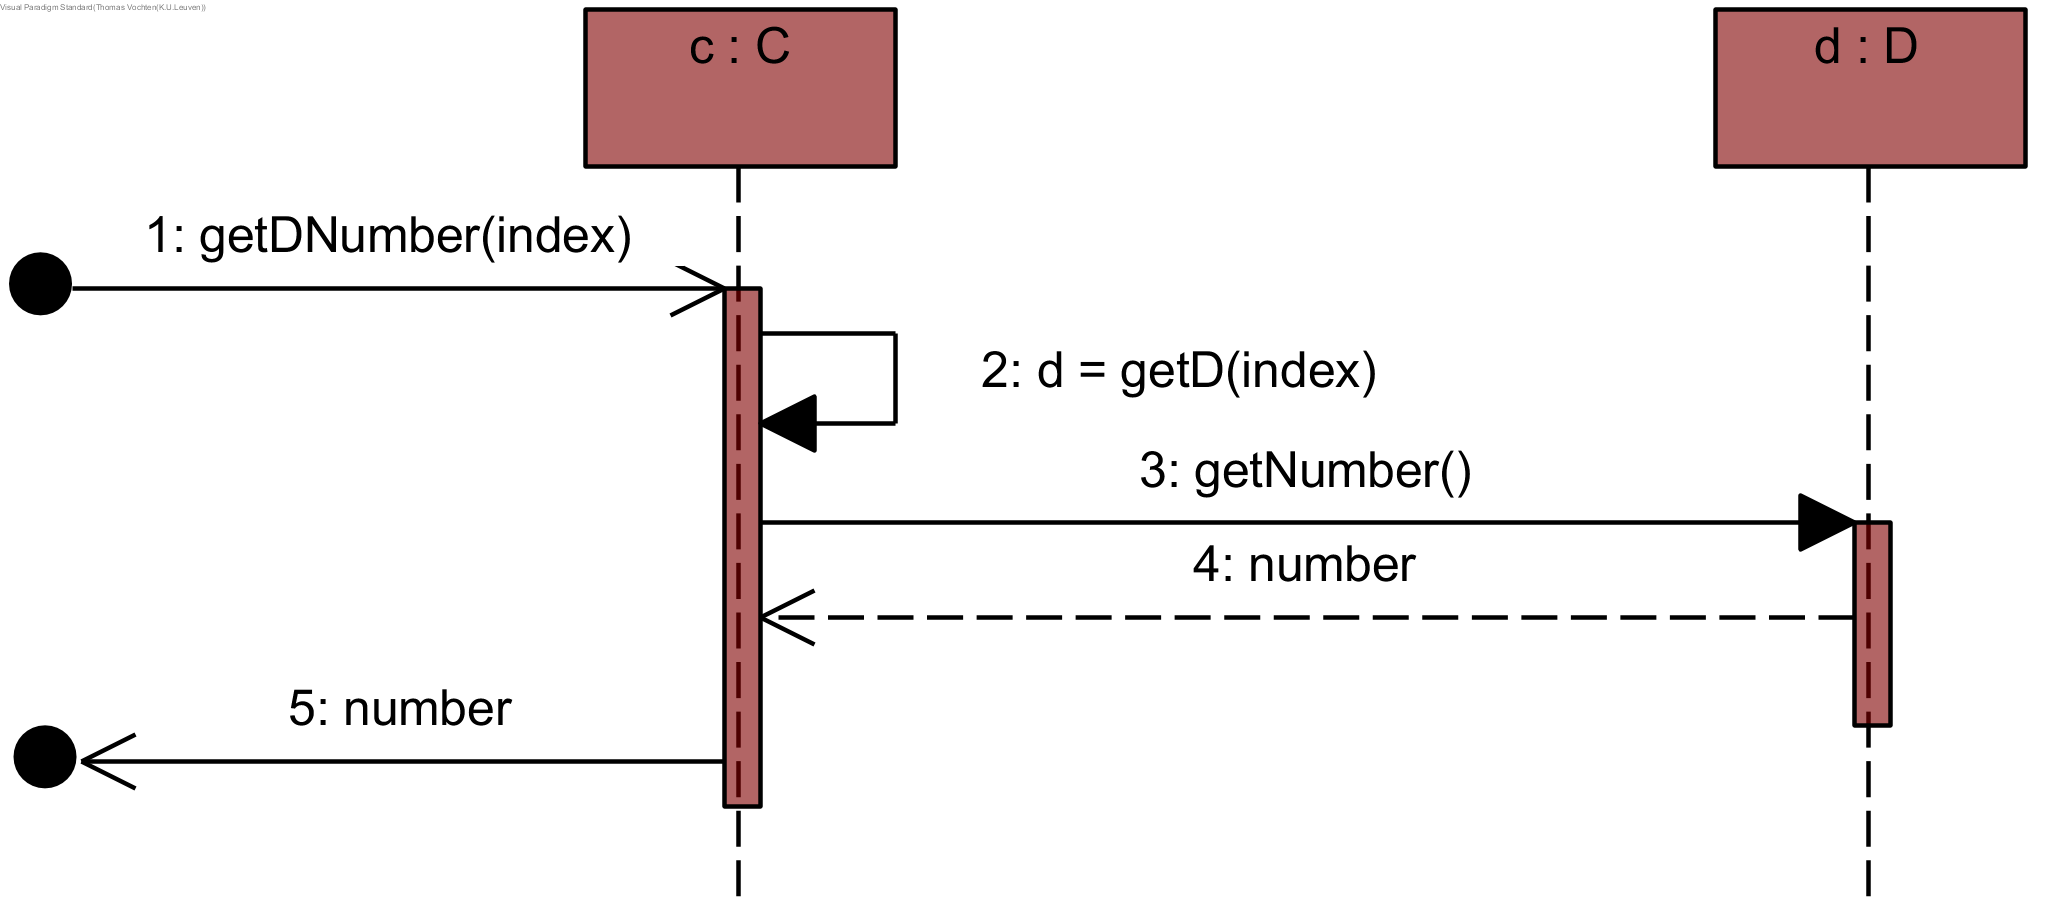
\includegraphics{intro/sd.png}
	\caption{Een voorbeeld van een sequentiediagram}
\end{figure}

Het toont hoe de juiste instantie van \textit{D} wordt opgehaald op basis van invoervariabele \textit{index} en hoe de waarde van het attribuut \textit{number} wordt doorgegeven aan instantie \textit{c}. \textit{c} geeft dan \textit{number} door als uitvoer van het sequentiediagram. Hoofdstuk \ref{sec:gedrag} legt meer in detail uit wat de betekenis is van de elementen die kunnen voorkomen in een sequentiediagram.

\subsection{Fysisch domein}

Artefacten in het fysisch domein bekijken het softwaresysteem vanuit het oogpunt van \textit{deployment}. \textit{Deployment} diagrammen geven weer hoe het systeem fysisch ge\"implementeerd wordt. Deze diagrammen benoemen fysische machines, geven aan welke verbindingen er bestaan tussen die machines en tonen welke concrete softwareartefacten draaien op elke machine.

\subsection{Modelbeheerdomein}

In dit domein beoogt men het beheer van de modellering van het systeem zelf. Tot dit domein behoren de \textit{package} diagrammen. Dit soort diagrammen organiseert de verscheidene soorten modelelementen van het softwaresysteem zoals klasses en \textit{use cases} in \textit{packages}. Een \textit{package} kan ook andere \textit{packages} bevatten. \textit{Package} diagrammen tonen welke \textit{packages} afhankelijk zijn van welke andere \textit{packages}. Zo krijgt men dus een beeld van welke modellen gebruik maken van elementen gedefinieerd in een ander model in hun beschrijving.

\section{Het kennisbanksysteem IDP}\label{sec:intro-idp}

Kennisbanksystemen\cite{1999XKSS} beogen het modelleren van kennis over een probleemdomein op een gestructureerde manier in een kennisbank. Ze bieden inferentiemethodes aan waarmee geredeneerd kan worden op die kennis. Zo kan een kennisbanksysteem nieuwe, meer precieze kennis afleiden of aantonen dat bepaalde eigenschappen gelden of niet gelden in de gegeven modellering van het domein. Ze laten ook het oplossen van concrete instanties van een probleem binnen het probleemdomein toe.

In deze masterproef gebruiken we IDP\cite{DeCatBroes2014PLaa}. In IDP zijn kennisbanken opgesteld in FO($\cdot$), een uitbreiding van predicatenlogica.

IDP bouwt verder op eerder werk in het onderzoeksdomein van het logisch programmeren. Het ondersteunt constructies gebaseerd op logisch programmeren, in het bijzonder inductieve definities, maar breekt ook met enkele fundamentele idee\"en uit dat paradigma. Logische theorie\"en opgesteld in FO($\cdot$) zijn geen uitvoerbare programma's---ze zijn beschrijvingen van kennis in het beschouwde probleemdomein. In IDP bestaat de fundamentele oplossingsstrategie voor problemen in een toepassingsdomein uit het specificeren van informatie over het domein in logica. De gebruiker past dan een vorm van inferentie toe om een antwoord te krijgen op concrete vragen geformuleerd in termen van het toepassingsdomein.

Bij het opstellen van logische theorie\"en ondersteunt IDP alle concepten uit de klassieke eerste-orde-predicatenlogica: Constanten, variabelen, predicaten, functies en existenti\"ele en universele kwantoren. IDP ondersteunt ook concepten die eerste-orde-predicantelogica uitbreiden. Concreet gaat het over de volgende vier concepten:

\begin{itemize}
	\item \textbf{Logische types}: Alle variabelen gebruikt in een logische zin hebben een type. Dit betekent ook dat alle argumenten van een predicaat en functie en het resultaat van een functie een type hebben.
	\item \textbf{Aggregaten}: Dit zijn de functies \textit{cardinaliteit}, \textit{som}, \textit{product}, \textit{minimum} en \textit{maximum}. De ontwerper specificeert \'e\'en variabele of een tupel van variabelen. Hij bindt die variabele of tupel dan in een logische zin. Als de ontwerper \'e\'en variabele specificeert, worden alle waarden die voldoen aan de logische zin als argument doorgegeven aan de aggregaatfunctie. Als de ontwerper een tupel specificeert, dan wordt voor elk tupel die voldoet aan de zin het eerste element doorgegeven aan de aggregaatfunctie.
	\item \textbf{Inductieve definities}: Dit is een mechanisme om de interpretatie van een predicaat of functie te defini\"eren analoog aan hoe een concept kan gedefinieerd worden in een recursieve definitie in de wiskunde of in verscheidene domeinen van de wetenschap.
	\item \textbf{Parti\"ele functies}: IDP laat toe om een functie te specificeren als \textit{partieel}. Dit betekent dat de functie niet noodzakelijk alle elementen van het domein afbeeldt op een element uit het codomein.
\end{itemize}

De inferentievormen die IDP ondersteunt zijn: Modelexpansie, wat een deels ingevulde structuur uitbreidt tot mogelijke modellen; bepalen of een structuur een model is voor een theorie en/of bepalen of een structuur kan uitgebreid worden tot een model voor de theorie; het vinden van optimale modellen gegeven een aggregate term; propagatie, wat gegeven een structuur en een theorie een preciezere structuur geeft die alle oplossingen behoudt; \textit{query}-inferentie, wat alle objecten die beantwoorden aan een bepaalde \textit{query} ophaalt uit een gegeven structuur; \textit{theorem proving} door middel van de functie \textit{entails(theory, theory)}; en progressie\"inferentie, wat de simulatie van dynamische systemen gemodelleerd in de lineaire tijdscalculus\cite{BogaertsBart2014Sdsu} toelaat.

De basisblokken van een specificatie in IDP zijn als volgt:

\begin{itemize}
	\item \textbf{Vocabularium}: Hier specificeert de ontwerper de logische types die bestaan in het beschouwd domein en de predicaten en functies over die logische types.
	\item \textbf{Theorie}: Hier schrijft de ontwerper zinnen in FO($\cdot$) die bepalen welke structuren over het beschouwde vocabularium modellen zijn. Indien de ontwerper een inconsistente theorie ontwerpt, zullen er geen modellen zijn.
	\item \textbf{Structuur}: De ontwerper vult hier de logische types gedefinieerd in het vocabularium in. \textit{Constructed types} hebben geen invulling nodig aangezien het vocabularium ze al volledig specificeert. De ontwerper kan ook voor \'e\'en of meerdere predicaten aangeven welke tupels wel of geen lid zijn. Hij kan ook voor \'e\'en of meerdere functies specificeren welke elementen uit het domein afgebeeld worden op welk element uit het codomein.
\end{itemize}

De ontwerper kan meerdere vocabularia, theorie\"en en structuren neerschrijven. Elke theorie en structuur kan wel maar de symbolen van \'e\'en vocabularium gebruiken.

Broes De Cat et al.\cite{DeCatBroes2014PLaa} geven een uitgebreidere inleiding tot IDP.

\section{Probleemstellingen}\label{sec:research-q}

Zoals aangehaald in sectie \ref{sec:situering}, kunnen er inconsistenties of onduidelijkheden sluipen in een klassediagram. Het kan ook dat het gedrag gemodelleerd in een sequentiediagram ingaat tegen bepaalde functionele eisen op het softwaresysteem.

\subsection{Probleemstellingen omtrent klassediagrammen}

We beschouwen twee categorie\"en van gebreken in een klassediagram:

\begin{itemize}
	\item \textbf{Inconsistenties:} Het klassediagram is zo opgebouwd dat geen enkele mogelijke toestand van de software kan beantwoorden aan de voorwaarden die worden opgelegd. Dit betekent dat het stuk van de software dat wordt beschreven in het diagram onmogelijk kan functioneren.
	\item \textbf{Kwaliteitsgebreken:} Deze gebreken hebben een negatieve impact op de kwaliteit van het softwareontwerp. Zo kunnen ze het bijvoorbeeld moeilijker maken om het diagram te begrijpen.
\end{itemize}

We onderzoeken hoe we klassediagrammen kunnen vertalen naar een voorstelling die ons toelaat om automatisch de consistentie van het diagram te controleren en om bepaalde soorten kwaliteitsgebreken op te sporen.

\subsection{Probleemstellingen omtrent sequentiediagrammen}

We willen het volgende uitvoeren voor sequentiediagrammen:

\begin{itemize}
	\item Het simuleren van het gedrag gemodelleerd in een bepaald stel sequentiediagrammen.
	\item Het verifi\"eren of de uitvoer van een sequentiediagram beantwoordt aan de vereisten opgelegd op de methode die dat sequentiediagram modelleert.
	\item Het verifi\"eren of het gedrag gemodelleerd in een stel sequentiediagrammen overeenkomt met gewenst gedrag in het beoogd softwaresysteem. Een voorbeeld van gewenst gedrag is dat een speler in een schaakspel maar \'e\'en stuk van zijn kleur mag bewegen per beurt.
\end{itemize}

We onderzoeken hoe we sequentiediagrammen kunnen vertalen naar een voorstelling die een uitvoering van het systeem kan simuleren. Met die voorstelling verifi\"eren we ook de uitvoer van sequentiediagrammen en of het gedrag van het systeem als geheel voldoet aan bepaalde eigenschappen.

\section{Verdere verloop van deze tekst}\label{sec:text-structure}

Hoofdstuk \ref{sec:literatuur} geeft een overzicht van literatuur omtrent het gebruik van logica om klassediagrammen en sequentiediagrammen voor te stellen.

Hoofdstuk \ref{sec:consistentie} beschrijft hoe we FO($\cdot$) gebruiken om klassediagrammen voor te stellen. We tonen aan dat we consistentie van een klassediagram kunnen verifi\"eren met modelexpansie. We kunnen enkele vormen van inconsistentie opsporen met \textit{theorem proving}, maar er is verder onderzoek nodig om op bepaalde andere vormen van inconsistentie te kunnen controleren. Dit hoofdstuk beschrijft ook een alternatieve voorstellingswijze die we gebruiken om bepaalde kwaliteitsgebreken op te sporen. We tonen aan dat we de aanwezigheid van losstaande klasses, \textit{many-to-many} associaties en onvoldoende nauw gespecificeerde bovengrenzen op een uiteinde van een associatie kunnen detecteren met modelexpansie.

\sloppy Hoofdstuk \ref{sec:gedrag} beschrijft hoe we sequentiediagrammen voorstellen in de lineaire tijdscalculus\cite{BogaertsBart2014Sdsu}, een methode om in FO($\cdot$) dynamische systemen te modelleren.

Hoofdstuk \ref{sec:evaluatie} evalueert ons vertalingsproces. We modelleren twee spellen, met voor elk spel een klassediagram en een stel sequentiediagrammen. Die diagrammen gebruiken we enerzijds om met progressie\"inferentie de spellen te simuleren en anderzijds om verificaties van gewenste eigenschappen uit te voeren met modelexpansie. Daarbij letten we op de rekentijd en het geheugengebruik. We tonen aan dat we de spellen Nim en Reversi elk kunnen modelleren in een klassediagram en een stel sequentiediagrammen. Met de theorie opgesteld volgens de regels beschreven in hoofdstukken \ref{sec:consistentie} en \ref{sec:gedrag} kunnen we een spelverloop van Nim simuleren. We nemen waar dat er relatief veel tijd en geheugen nodig is om deze simulaties uit te voeren. Verder tonen we aan dat we kunnen verifi\"eren of de uitvoer van een sequentiediagram voldoet aan bepaalde eisen op de methode gemodelleerd in dat sequentiediagram. Als laatste tonen we aan dat we kunnen controleren of de sequentiediagrammen garanderen dat een spelbeurt in Nim altijd verloopt zoals voorgeschreven door de spelregels.

Gemotiveerd door de inzichten verkregen in hoofdstuk \ref{sec:evaluatie}, geeft hoofdstuk \ref{sec:decl-seq} een aanzet om de ontwerptaal beschikbaar voor sequentiediagrammen uit te breiden met declaratieve constructies. Het doel is om ervoor te zorgen dat er significant minder berichten nodig zijn in een sequentiediagram om het gedrag van een methode te specificeren. We modelleren Nim opnieuw met deze constructies en tonen aan dat er significant minder rekentijd en geheugen nodig is om modelexpansie en simulatie door middel van progressie\"inferentie uit te voeren.

Hoofdstuk \ref{sec:conclusie} geeft een besluit en een aanzet tot verder onderzoek.